%%%%%%%%%%%%%%%%%%%%%%%%%%%%%%%%%%%%%%%%%%%%%%%%%%%%%%%%%%%%
%%%%%%%%%%%%%%%%%%%%%%%%%%%%%%%%%%%%%%%%%%%%%%%%%%%%%%%%%%%%
\chapter{The Wako-Saito-Mu{\~n}oz-Eaton Model for Protein Folding
%Protein Folding Problem
}
\label{chap:wsme-model}
\nopagebreak
%%%%%%%%%%%%%%%%%%%%%%%%%%%%%%%%%%%%%%%%%%%%%%%%%%%%%%%%%%%%
%%%%%%%%%%%%%%%%%%%%%%%%%%%%%%%%%%%%%%%%%%%%%%%%%%%%%%%%%%%%

In this chapter we introduce the Wako-Saito-Mu{\~n}oz-Eaton (WMSE) model and its application to the protein folding 
problem.
After reviewing the main features of the model, we address the calculations of
both thermodynamics and kinetics observables that are relevant in experimental
studies of the protein folding process, both for ensemble and for
single-molecule experiments.

%%%%%%%%%%%%%%%%%%%%%%%%%%%%%%%%%%%%%%%%%%%%%%%%%%%%%%%%%%%
\section{Methods}
\label{sec:methods}
\subsection{Model}

WSME is a native-centric model \cite{Ueda1978}, i.e. it relies on the knowledge of
the native state of the protein to describe its equilibrium and kinetics.
Its binary variables $m_k$, accounting for the local backbone and side chain
angles, describe the state of each residue  $k \in [1, N]$
 as ordered (native,  $m_k=1$) and disordered
(unfolded, $m_k=0$). Since the latter state allows a much larger number of
microscopic realizations than the former, an entropic cost  $q_k$ is
given to the ordering of residue $k$.

The model is described by the 
effective Hamiltonian (indeed, a free energy, where the solvent and the fast
degrees of freedom have been integrated out):
\begin{equation}
H =  - \sum_{i=1}^{N-1}\sum_{j=i+1}^{N}
\epsilon_{i,j} \Delta_{i,j} \prod_{k=i}^{j} m_k
+  \sum_{k=1}^{N} (q_k  T +  \alpha c) m_k  ,
\label{Hamiltonian}
\end{equation}
where $N$ is the number of residues  in the molecule and $T$ the absolute
temperature. The product ${\prod_{k=i}^j} m_k$ takes value 1 if and only
if all the peptide bonds from $i$ to $j$ are in the native state: indeed, within
the model such interaction is ensured only if all the main chain angles of the
residues between $i$ and $j$ are in the correct folded conformation.
Non--native interactions are
disregarded, while native interactions are accounted for in the contact matrix
$\Delta_{i,j}$, which counts the number of contacts between atoms of
non--contiguous residues $i$ and $j$ in the native structure, according to a
cut-off distance criterion. In the following, we will use the contact map
calculated from the crystal structure of Myotrophin deposited in the Protein
Data Bank  (PDB code: 2myo), considering that a contact is established if any
two atoms (including hydrogen atoms) from residues $i$ and $j$ are found at a
distance less than 3.5 $\mathring{A}$.  Figure \ref{fig:map} reports the
resulting contact map.

\begin{figure}
\centering
\includegraphics[width=0.4\textwidth,angle=-90]{./img/wsme/allH-map-square.eps}
\caption{\label{fig:map}Weighted contact map for Myotrophin (2myo). The
area of each circle is proportional to the weight of the contact between
residues $i$ and $j$, in terms of the number of inter-atomic interactions.
Inter-atomic contacts are established if two atoms belonging to residue $i$ and
$j$ respectively are nearer then 3.5 $\mathring{A}$.
Darker areas represent contacts between residues that
belong to helices.}
\end{figure}

The expression above differs from the original one for the  last term,
accounting for the interaction between the denaturant, usually urea,
and the protein backbone
(as suggested by \citet{Auton2007}, and also in agreement
with the choice in Ref.~\cite{Ferreiro2008}), where $c$ represents the urea
molar concentration and $\alpha$ is a new parameter.

\paragraph{Setting the Values of the Parameters.}
For the sake of simplicity,  we take homogeneous parameters $\epsilon_{i,j} =
\epsilon$, $q_i=q$, for each $i$ and $j$, with $\epsilon,q>0$, to model the wild
type protein.
We use the experimental thermodynamics data to adjust the parameters: we set
$q=2 R$, as in \cite{Zamparo2006a},
and find $ \epsilon$, and $\alpha$ by fitting the equilibrium experimental data
of Refs.~\cite{Mosavi2002a,Lowe2007a} for the wild type species. 
We first
calculate the native and unfolded baselines $n(z)$ and $u(z)$, where $z$ is the
temperature or denaturant concentration, respectively, from the data, following
the usual experimental procedure, and consider the order parameter:
\begin{equation}
 p(z)=\frac{m(z)-u(z)}{n(z)-u(z)}\,,
\label{eq:ordpar_p}
\end{equation}
normalized between zero (unfolded) and one (native). 
Here $m(z)$ is the equilibrium average fraction of folded residues, defined  in
Equation~\ref{eq:avenatfrac}.
Then, we adjust the $\epsilon$ parameter, imposing that the temperature $T_m$ at
which $p(T_m)=0.5$ coincides with the experimental mid-folding temperature
$T_m=327$~K . Then, we do the same for the $\alpha$ parameter, imposing that
$p(c_m)=0.5$ at the experimental mid-folding denaturant molar concentration
$c_m=3.2$. The resulting values of the parameters are used in the whole study,
for both wild type and mutated species.
The results are reported in figure \ref{fig:den-fit}.
\begin{figure}
\centering
\subfigure[{\protect [Urea]}]{
%\includegraphics[width=0.26\textwidth,angle=-90]{./img/wsme/den-fit-chem.eps}}
\resizebox{0.4\textwidth}{!}{\sffamily% GNUPLOT: LaTeX picture with Postscript
\begingroup
  \makeatletter
  \providecommand\color[2][]{%
    \GenericError{(gnuplot) \space\space\space\@spaces}{%
      Package color not loaded in conjunction with
      terminal option `colourtext'%
    }{See the gnuplot documentation for explanation.%
    }{Either use 'blacktext' in gnuplot or load the package
      color.sty in LaTeX.}%
    \renewcommand\color[2][]{}%
  }%
  \providecommand\includegraphics[2][]{%
    \GenericError{(gnuplot) \space\space\space\@spaces}{%
      Package graphicx or graphics not loaded%
    }{See the gnuplot documentation for explanation.%
    }{The gnuplot epslatex terminal needs graphicx.sty or graphics.sty.}%
    \renewcommand\includegraphics[2][]{}%
  }%
  \providecommand\rotatebox[2]{#2}%
  \@ifundefined{ifGPcolor}{%
    \newif\ifGPcolor
    \GPcolortrue
  }{}%
  \@ifundefined{ifGPblacktext}{%
    \newif\ifGPblacktext
    \GPblacktexttrue
  }{}%
  % define a \g@addto@macro without @ in the name:
  \let\gplgaddtomacro\g@addto@macro
  % define empty templates for all commands taking text:
  \gdef\gplbacktext{}%
  \gdef\gplfronttext{}%
  \makeatother
  \ifGPblacktext
    % no textcolor at all
    \def\colorrgb#1{}%
    \def\colorgray#1{}%
  \else
    % gray or color?
    \ifGPcolor
      \def\colorrgb#1{\color[rgb]{#1}}%
      \def\colorgray#1{\color[gray]{#1}}%
      \expandafter\def\csname LTw\endcsname{\color{white}}%
      \expandafter\def\csname LTb\endcsname{\color{black}}%
      \expandafter\def\csname LTa\endcsname{\color{black}}%
      \expandafter\def\csname LT0\endcsname{\color[rgb]{1,0,0}}%
      \expandafter\def\csname LT1\endcsname{\color[rgb]{0,1,0}}%
      \expandafter\def\csname LT2\endcsname{\color[rgb]{0,0,1}}%
      \expandafter\def\csname LT3\endcsname{\color[rgb]{1,0,1}}%
      \expandafter\def\csname LT4\endcsname{\color[rgb]{0,1,1}}%
      \expandafter\def\csname LT5\endcsname{\color[rgb]{1,1,0}}%
      \expandafter\def\csname LT6\endcsname{\color[rgb]{0,0,0}}%
      \expandafter\def\csname LT7\endcsname{\color[rgb]{1,0.3,0}}%
      \expandafter\def\csname LT8\endcsname{\color[rgb]{0.5,0.5,0.5}}%
    \else
      % gray
      \def\colorrgb#1{\color{black}}%
      \def\colorgray#1{\color[gray]{#1}}%
      \expandafter\def\csname LTw\endcsname{\color{white}}%
      \expandafter\def\csname LTb\endcsname{\color{black}}%
      \expandafter\def\csname LTa\endcsname{\color{black}}%
      \expandafter\def\csname LT0\endcsname{\color{black}}%
      \expandafter\def\csname LT1\endcsname{\color{black}}%
      \expandafter\def\csname LT2\endcsname{\color{black}}%
      \expandafter\def\csname LT3\endcsname{\color{black}}%
      \expandafter\def\csname LT4\endcsname{\color{black}}%
      \expandafter\def\csname LT5\endcsname{\color{black}}%
      \expandafter\def\csname LT6\endcsname{\color{black}}%
      \expandafter\def\csname LT7\endcsname{\color{black}}%
      \expandafter\def\csname LT8\endcsname{\color{black}}%
    \fi
  \fi
  \setlength{\unitlength}{0.0500bp}%
  \begin{picture}(7200.00,5040.00)%
    \gplgaddtomacro\gplbacktext{%
      \csname LTb\endcsname%
      \put(660,400){\makebox(0,0)[r]{\strut{}-0.2}}%
      \put(660,1028){\makebox(0,0)[r]{\strut{} 0}}%
      \put(660,1657){\makebox(0,0)[r]{\strut{} 0.2}}%
      \put(660,2285){\makebox(0,0)[r]{\strut{} 0.4}}%
      \put(660,2914){\makebox(0,0)[r]{\strut{} 0.6}}%
      \put(660,3542){\makebox(0,0)[r]{\strut{} 0.8}}%
      \put(660,4171){\makebox(0,0)[r]{\strut{} 1}}%
      \put(660,4799){\makebox(0,0)[r]{\strut{} 1.2}}%
      \put(780,200){\makebox(0,0){\strut{} 0}}%
      \put(1790,200){\makebox(0,0){\strut{} 1}}%
      \put(2800,200){\makebox(0,0){\strut{} 2}}%
      \put(3810,200){\makebox(0,0){\strut{} 3}}%
      \put(4819,200){\makebox(0,0){\strut{} 4}}%
      \put(5829,200){\makebox(0,0){\strut{} 5}}%
      \put(6839,200){\makebox(0,0){\strut{} 6}}%
    }%
    \gplgaddtomacro\gplfronttext{%
      \csname LTb\endcsname%
      \put(5936,4636){\makebox(0,0)[r]{\strut{}exp}}%
      \csname LTb\endcsname%
      \put(5936,4436){\makebox(0,0)[r]{\strut{}fit}}%
    }%
    \gplbacktext
    \put(0,0){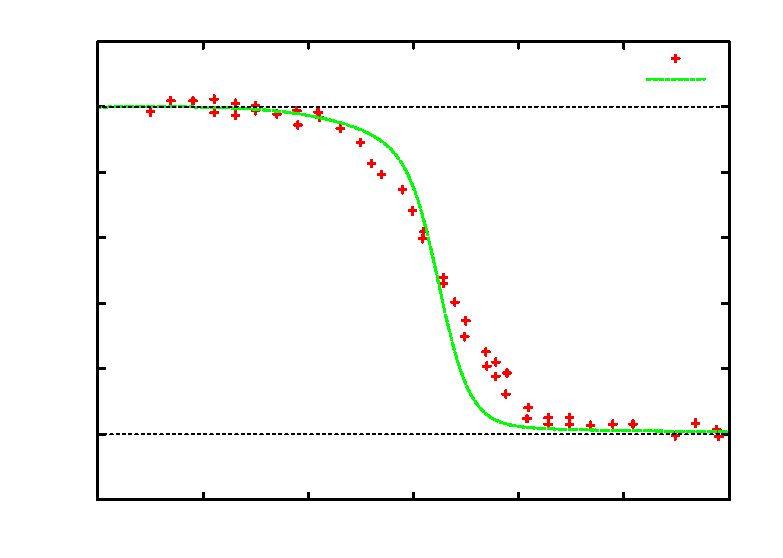
\includegraphics{img/wsme/den-fit-chem-lw2}}%
    \gplfronttext
  \end{picture}%
\endgroup
}}
\subfigure[Temperature]{
%\includegraphics[width=0.26\textwidth,angle=-90]{./img/wsme/den-fit-therm.eps}}
\resizebox{0.4\textwidth}{!}{\sffamily% GNUPLOT: LaTeX picture with Postscript
\begingroup
  \makeatletter
  \providecommand\color[2][]{%
    \GenericError{(gnuplot) \space\space\space\@spaces}{%
      Package color not loaded in conjunction with
      terminal option `colourtext'%
    }{See the gnuplot documentation for explanation.%
    }{Either use 'blacktext' in gnuplot or load the package
      color.sty in LaTeX.}%
    \renewcommand\color[2][]{}%
  }%
  \providecommand\includegraphics[2][]{%
    \GenericError{(gnuplot) \space\space\space\@spaces}{%
      Package graphicx or graphics not loaded%
    }{See the gnuplot documentation for explanation.%
    }{The gnuplot epslatex terminal needs graphicx.sty or graphics.sty.}%
    \renewcommand\includegraphics[2][]{}%
  }%
  \providecommand\rotatebox[2]{#2}%
  \@ifundefined{ifGPcolor}{%
    \newif\ifGPcolor
    \GPcolortrue
  }{}%
  \@ifundefined{ifGPblacktext}{%
    \newif\ifGPblacktext
    \GPblacktexttrue
  }{}%
  % define a \g@addto@macro without @ in the name:
  \let\gplgaddtomacro\g@addto@macro
  % define empty templates for all commands taking text:
  \gdef\gplbacktext{}%
  \gdef\gplfronttext{}%
  \makeatother
  \ifGPblacktext
    % no textcolor at all
    \def\colorrgb#1{}%
    \def\colorgray#1{}%
  \else
    % gray or color?
    \ifGPcolor
      \def\colorrgb#1{\color[rgb]{#1}}%
      \def\colorgray#1{\color[gray]{#1}}%
      \expandafter\def\csname LTw\endcsname{\color{white}}%
      \expandafter\def\csname LTb\endcsname{\color{black}}%
      \expandafter\def\csname LTa\endcsname{\color{black}}%
      \expandafter\def\csname LT0\endcsname{\color[rgb]{1,0,0}}%
      \expandafter\def\csname LT1\endcsname{\color[rgb]{0,1,0}}%
      \expandafter\def\csname LT2\endcsname{\color[rgb]{0,0,1}}%
      \expandafter\def\csname LT3\endcsname{\color[rgb]{1,0,1}}%
      \expandafter\def\csname LT4\endcsname{\color[rgb]{0,1,1}}%
      \expandafter\def\csname LT5\endcsname{\color[rgb]{1,1,0}}%
      \expandafter\def\csname LT6\endcsname{\color[rgb]{0,0,0}}%
      \expandafter\def\csname LT7\endcsname{\color[rgb]{1,0.3,0}}%
      \expandafter\def\csname LT8\endcsname{\color[rgb]{0.5,0.5,0.5}}%
    \else
      % gray
      \def\colorrgb#1{\color{black}}%
      \def\colorgray#1{\color[gray]{#1}}%
      \expandafter\def\csname LTw\endcsname{\color{white}}%
      \expandafter\def\csname LTb\endcsname{\color{black}}%
      \expandafter\def\csname LTa\endcsname{\color{black}}%
      \expandafter\def\csname LT0\endcsname{\color{black}}%
      \expandafter\def\csname LT1\endcsname{\color{black}}%
      \expandafter\def\csname LT2\endcsname{\color{black}}%
      \expandafter\def\csname LT3\endcsname{\color{black}}%
      \expandafter\def\csname LT4\endcsname{\color{black}}%
      \expandafter\def\csname LT5\endcsname{\color{black}}%
      \expandafter\def\csname LT6\endcsname{\color{black}}%
      \expandafter\def\csname LT7\endcsname{\color{black}}%
      \expandafter\def\csname LT8\endcsname{\color{black}}%
    \fi
  \fi
  \setlength{\unitlength}{0.0500bp}%
  \begin{picture}(7200.00,5040.00)%
    \gplgaddtomacro\gplbacktext{%
      \csname LTb\endcsname%
      \put(660,400){\makebox(0,0)[r]{\strut{}-0.2}}%
      \put(660,1028){\makebox(0,0)[r]{\strut{} 0}}%
      \put(660,1657){\makebox(0,0)[r]{\strut{} 0.2}}%
      \put(660,2285){\makebox(0,0)[r]{\strut{} 0.4}}%
      \put(660,2914){\makebox(0,0)[r]{\strut{} 0.6}}%
      \put(660,3542){\makebox(0,0)[r]{\strut{} 0.8}}%
      \put(660,4171){\makebox(0,0)[r]{\strut{} 1}}%
      \put(660,4799){\makebox(0,0)[r]{\strut{} 1.2}}%
      \put(780,200){\makebox(0,0){\strut{} 270}}%
      \put(1386,200){\makebox(0,0){\strut{} 280}}%
      \put(1992,200){\makebox(0,0){\strut{} 290}}%
      \put(2598,200){\makebox(0,0){\strut{} 300}}%
      \put(3204,200){\makebox(0,0){\strut{} 310}}%
      \put(3810,200){\makebox(0,0){\strut{} 320}}%
      \put(4415,200){\makebox(0,0){\strut{} 330}}%
      \put(5021,200){\makebox(0,0){\strut{} 340}}%
      \put(5627,200){\makebox(0,0){\strut{} 350}}%
      \put(6233,200){\makebox(0,0){\strut{} 360}}%
      \put(6839,200){\makebox(0,0){\strut{} 370}}%
    }%
    \gplgaddtomacro\gplfronttext{%
      \csname LTb\endcsname%
      \put(5936,4636){\makebox(0,0)[r]{\strut{}exp}}%
      \csname LTb\endcsname%
      \put(5936,4436){\makebox(0,0)[r]{\strut{}fit}}%
    }%
    \gplbacktext
    \put(0,0){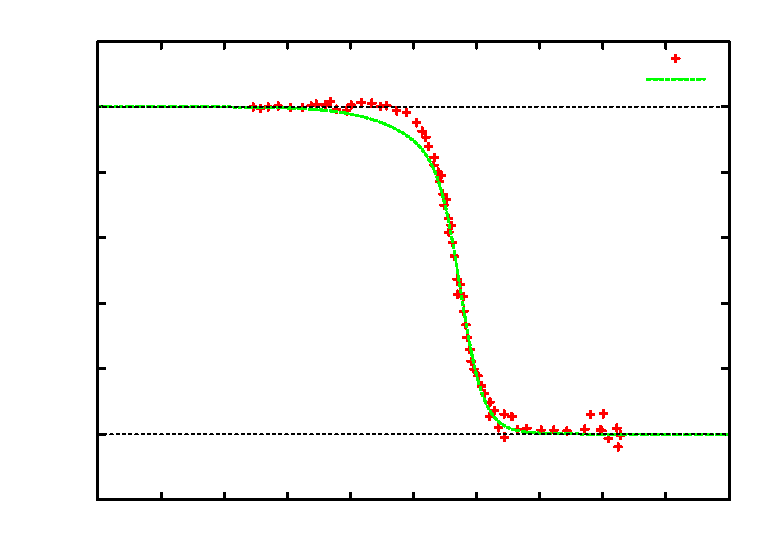
\includegraphics{img/wsme/den-fit-therm-lw2}}%
    \gplfronttext
  \end{picture}%
\endgroup
}}
\caption{
\label{fig:den-fit} 
Fit of the order parameter $p(z)$ from the WSME model to the experimental data
for (a) urea-induced denaturation{\protect \cite{Lowe2007a}} and (b) thermal
denaturation{\protect \cite{Mosavi2002a}}.
Parameters values are: $\varepsilon=0.2276$ kJ/mol, %$q=0.016628944$ 
$q=0.0166$  kJ/(K mol), $\alpha=0.208$ kJ/([urea] mol)}
\end{figure}

\paragraph{Mutations.}
Mutations are mimicked by perturbing a group of contacts, of one or more
residues as detailed below, through the addition of a $\Delta \epsilon_{i,j}$
to the corresponding interactions.
To make comparison easier, the same total
perturbation of $\varepsilon_\text{tot}$=9.21 kJ/mol, comparable with those reported
in Ref.~\cite{Lowe2007a},  is introduced for all mutants, so that the $\Delta
\epsilon_{i,j}$ will vary between  mutants, according to the number of affected
contacts, resulting as follow:
\begin{equation}
\Delta\epsilon_{i,j}=\varepsilon_\text{tot}\frac{n^\text{ct}_{i,j}}{n^\text{ct}_\text{tot}}
\end{equation}
where the number of affected contacts between residue $i$ and residue $j$ is 
$n^\text{ct}_{i,j}$ and $n^\text{ct}_\text{tot}$ is the total amount of affected
contacts.

The list of analysed mutations is reported in Table~\ref{table:mutations}, and
was selected to probe different regions of residues and different distances
between contacting residues.
\begin{table}
\centering
\begin{tabular}{ c | l }
\hline \hline 
name & description \\
\hline
WT		& wild type protein\\
$S_{1,2}$	& contacts of residues [5\dots10] with residues [17,18]\\
$S_{3}$		& contacts of residue 32\\
$S_{3,4}$	& contacts of residues [36\dots44] with residues [49\dots56]\\
$S_{1,4}$	& contacts of residues [9\dots18] with residues [45\dots53]\\
$S_{5,6}$	& contacts of residues [71\dots76] with residues [82\dots88]\\
$S_{3,6}$	& contacts of residues [42\dots52] with residues [78\dots83]\\
$S_{7}$		& contacts of residue [103] with residues [94\dots101]\\
$S_{7,8}$	& contacts of residues [104,105] with residues [113,114]\\
$S_{5,8}$	& contact  between residue 76 and residue 113\\
\hline \hline
\end{tabular}
\caption{\label{table:mutations}  List of mutations analysed in this work. The
same total destabilization of 9.21 kJ/mol was used in all cases, adapting the
individual $\Delta \epsilon_{i,j}$ of each contact. The indices $m,n$ in
$S_{m,n}$ specify the helices involved in the mutated contacts. $S_3$ actually
affects a loop residue, close to helix 3.}
\end{table}


We also analyse the case of some multiple mutations that have been investigated
experimentally in Ref.~\cite{Lowe2007} to test the two-pathway interpretation.
In order to compare our model to those results, we have simulated the effect of
those mutations applying a stabilizing or destabilizing perturbation (whose
energy is taken from Ref.~\cite{Lowe2007}) equally spread on
all the contacts of the mutated residues. The following
mutants are considered:
\begin{itemize}
\item E17V/D20L ($\Delta\Delta G_\textrm{eq.}= -7.12 - 2.09$ kJ/mol C: a stabilized mutant)
\item A9G ($\Delta\Delta G_\textrm{eq.}= 10.38$ kJ/mol C)
\item A115G ($\Delta\Delta G_\textrm{eq.}= 3.39$ kJ/mol C)
\item A115G/A9G
\item A115G/E17V/D20L
\item A9G/E17V/D20L/A115G
\end{itemize}

Multiple mutations are considered as independent, and the corresponding
energetic perturbation is applied to each point mutation separately, so that,
e.g., $\Delta \Delta G_{A115G/A9G}= \Delta \Delta G_{A115G} + \Delta \Delta
G_{A9G}$.

%%----------------------------------------------------------
\subsection{Thermodynamics}
The equilibrium values of all thermodynamic quantities  are calculated resorting
to the exact solution of the model \cite{Bruscolini2002,Pelizzola2005}. In
particular, we will study the fraction of native residues:
\begin{equation}
m=\frac{1}{N} \sum_{i=1}^{N} \langle m_i \rangle\,,
\label{eq:avenatfrac}%
\end{equation}
We can introduce the reaction coordinate $\rho=\frac M N$ as the fraction of native
residues $M$.
Free-energy profiles can be defined as a function of $\rho$:
\begin{equation}
F(\rho)=-RT \log{Z_\rho}\,,
\label{eq:fprofile} 
\end{equation}
where $Z_\rho=\sum'_{\lbrace m_{i}\rbrace} \exp{(- H/RT)}$, and the sum 
$\sum' (\bullet)$ is
restricted to the states with a fixed number of native residues $\sum_i m_i=M$.
The $Z_\rho$ can be easily calculated within the framework of the exact solution
mentioned above.

Finally, we will study the average values  
\begin{equation}
\mu_{i,j} = \langle m_{i,j} \rangle \,,
\label{eq:mu-strings}
\end{equation}
and
\begin{equation}
 \nu_{i,j} = \langle  (1-m_{i-1}) m_{i,j}  (1-m_{j+1}) \rangle\,,
\label{eq:nu-cappedstrings}
\end{equation}
of  the products $m_{i,j}=\prod_{k=i}^j m_k$. This product can assume only
values one or zero, meaning that the whole string from residue $i$ to residue
$j$ is respectively completely native or not. 
In this framework, $\mu_{i,j}$ represents the equilibrium probability that
the region between $i$ and $j$ is native, while $\nu_{i,j}$ represents the
probability that the same region is
capped by unfolded residues, thus representing an isolated native region.


%%----------------------------------------------------------
\subsection{Kinetics}

 
The kinetic evolution of the model outside the equilibrium is described through a
discrete--time master equation, $p_{t+1}(x) = \sum_{x'} W(x' \to x) p_t(x)$, 
for the probability distribution
$p_t(x)$ at time $t$, where $x = \{ m_k, \,k = 1, \ldots N \}$ denotes
the state of the system. 
Notice that this expression is not amenable to analytical treatment (even
if an accurate semi-analytical
approximation exists \cite{Zamparo2006,Zamparo2006a}), since by construction
$W(x' \to x)$ is a $2^N \times 2^N$ matrix.


In this work the kinetics will be studied by means of Monte Carlo simulations: as in
previous works \cite{Zamparo2006,Zamparo2006a}, the transition matrix $W$ is
specified by a single bond flip Metropolis rule, which implies that a flip is
accepted or rejected according to its equilibrium probability, at the
temperature and denaturant concentration specified for the simulation.
In order to study separately the folding and unfolding kinetics we fix folding
condition (T=293.15 K, $c$=0) and unfolding
conditions (T=293.15 K, $c$=12). 
The system is prepared in a initial state far from equilibrium and this is
defined as a random configuration extracted with the infinite temperature equilibrium
probability in the folding case, so that the initial
and final fraction of native residues are $ m(t=0)=0.12$ %$ m(t=0)=0.119$ 
and %$m(t=\infty)=0.966$
$m(t=\infty)=0.97$ respectively, for the wild type protein (slightly different
values are obtained for the mutants).
In unfolding simulations, the system is prepared in a
fully native state ($m_i=1$ for each $i$), while $m(t=\infty)=0.0047$,
%$m(t=\infty)=0.00468$
for the wild type protein. 


We study the relaxation of the average fraction of native residues $m(t)$: at
each time, the average is formally calculated as in Equation~(\ref{eq:avenatfrac}),
but with the $\langle \bullet \rangle$ now indicating the average over  $\cal N$
single molecule simulations, that is, over an ensemble  of $\cal N$ molecules.
We choose  $\cal N$=2000 as a reasonable trade-off between detecting a neat
signal and reducing simulation time.  We fit $m(t)$  with one- or
two-exponential expressions, namely:
\begin{equation}
m(t)=m_{eq}(T,c) + c_1 e^{-k_1 t} \,,
\label{eq:1expfit} 
\end{equation}
or
\begin{equation}
m(t)=m_{eq}(T,c) + c_1 e^{-k_1 t} + c_2 e^{-k_2 t}\,,
\label{eq:2expfit} 
\end{equation}
where $m_{eq}(T,c)$ is the equilibrium value at the temperature  $T$ and
denaturant concentration $c$, obtained from the thermodynamics calculations. The
fitting parameters are the rates $k_i$ and the corresponding amplitude $c_i$.

\paragraph{Pathways Heterogeneity.}
In order to characterize the folding and unfolding pathways, we rely on the
secondary structure formation (denaturation) times. Myotrophin is composed by
eight helices (7 $\alpha$-helices and one $\pi$-helix) which are supposed to be
partially stable structures, as stabilized by internal hydrogen bonds.
These can then be interpreted as fundamental structural motifs.
To characterize the helices folding and denaturation in order to find a common
behaviour, we define the regions $h_l=(i_l,j_l)$, $l=1,\dots,8$
corresponding to the eight helices of the native Myotrophin structure, 
as well as the regions
$R_{\alpha,\beta}$ encompassing the fragment from helix $\alpha$ to $\beta$
inclusive (that is, from residue $i_{\alpha}$ where helix $\alpha$ begins, to
residue $j_{\beta}$ where helix $\beta$ ends).
After defining the folding time $t_f$ as the first passage time (in Monte Carlo
steps) through the
state with all the helices formed ($R_{1,8}$), we identify, for each single
molecule simulation of the folding process, the stabilization time
$t_{\alpha,\beta}^{(f)}$ of each region $R_{\alpha,\beta}$ as the last time it
turns completely native (thus, waiting for all the fluctuations to fade away).
This choice is a natural generalization of that proposed in
Ref.~\cite{Zamparo2009}, to the present case with many elements of secondary
structure: notice indeed  that, due to the model characteristics, the
stabilization of $R_{\alpha,\beta}$ in the native conformation is a necessary
and sufficient condition for the formation of contacts between helix $\alpha$
and $\beta$ (if any), as well as between all pairs of helices $k$,$l$, with
$\alpha \le k < l \le \beta$. The determination of $t_{\alpha,\beta}^{(f)}$ for
all regions allows us to determine pathways in the secondary structure
formation, and to identify two main pathways in the folding and unfolding of
Myotrophin (see Chapter \ref{chap:wsme-results} below).
% Indeed the same quantities $t^{(f)}_{a,b}$ are used also to characterize the
% unfolding, since in this case they signal the last time the region $R_{a,b}$
% was found completely folded, before the undolfing time $t_u$ NOOOOOO!.
%\begin{minipage}{\textwidth}
%\tiny
%MC
%\colorbox{red}{DKEFMWALKN}
%GD
%\colorbox{red}{LDEVKDYV}
%AKGEDVNRTLEGGRKPL
%\colorbox{red}{HYAADC}
%GQL
%\colorbox{red}{EILEFLLLK}
%GADINAPDKHHIT
%\colorbox{red}{PLLSAV}
%YEGHV
%\colorbox{red}{SCVKLLL}
%SKGADKTVKGPDG
%\colorbox{red}{LTALE}
%ATDNQA
%\colorbox{red}{IKAL}
%LQ
%\end{minipage}


We define also the probability of a given region $R_{\alpha,\beta}$ to fold
before a different $R_{\alpha',\beta'}$, relying on the folding times as defined
before.
This can induce interpretation errors in case of wildly fluctuating elements
that translate in a measured late stabilization and an artificial ordering of
the helices folding times.
%We also record the joint probabilities that two non-overlapping regions  are
%native at the same time, for each single-molecule simulation. This is to avoid
%that a wildly fluctuating element, with a late stabilization,  induce an
%artificial ordering along the pathway. ??perche? se una elica fluttua la
%relativa probabilita di formarsi dopo le altre sara alta, ingannando in ogni
%caso l'sosservatore.
We have observed, in any case, that the
only elements in Myotrophin for which strong  fluctuations could induce an
interpretation
problem are the first and last helix, which on the other hand turn out to be
unimportant for pathway determination (see Chapter \ref{chap:wsme-results}). For the
other helices, we observe that local fluctuations can indeed invert the order by
which a region is stabilized,  in different single-molecule runs, starting from
its constituent elements. 
However, the difference in stabilization times among
the latter is small, allowing to group clearly which elements stabilize
basically altogether in the folding process.

We do the same for the unfolding simulations: now the unfolding time $t_u$ is
defined as the first passage time in a state with $m<0.09$, and for each single
molecule simulation, we record the last time $t_{\alpha,\beta}^{(u)}$ in which
each region $R_{\alpha,\beta}$ switches from the native to unfolded state.


